\documentclass[11pt]{article}
\usepackage[english]{babel}
\usepackage{amsmath}
\usepackage{amsthm}
\usepackage{graphicx}
\usepackage{subcaption}
\usepackage{booktabs}
\usepackage{float}
\usepackage[left=25mm, top=25mm, bottom=30mm, right=25mm]{geometry}
\usepackage[colorlinks=true, linkcolor=blue, urlcolor=cyan]{hyperref}

\title{COL774: Assignment 3}
\author{Sayam Sethi}
\date{October 2021}

\begin{document}

\maketitle

\tableofcontents

\section{Random Forests}

\subsection{Grid Search}
The best model obtained is for the following parameters:
\begin{itemize}
  \item \textbf{n\_estimators}: 450
  \item \textbf{max\_features}: 0.3
  \item \textbf{min\_samples\_split}: 6
\end{itemize}

\subsection{Paramter Sensitivity Analysis}
\subsubsection{n\_estimators}
\begin{figure}[H]
  \centering
  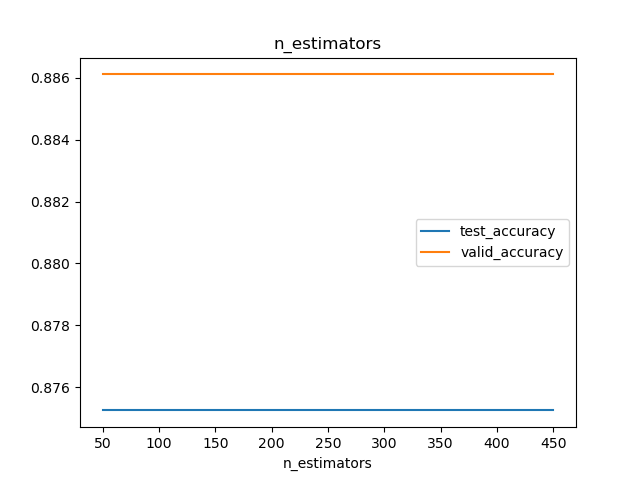
\includegraphics[width=0.6\textwidth]{Q1/output/d_n.png}
  \caption{Plot of the effect of n\_estimators on the accuracy of the model}
\end{figure}
The validation accuracy increases on increasing the number of estimators. However the test accuracy drops slightly. However the training accuracy increases with increasing the number of estimators. Therefore, the model overfits with larger number of estimators.

\subsubsection{max\_features}
\begin{figure}[H]
  \centering
  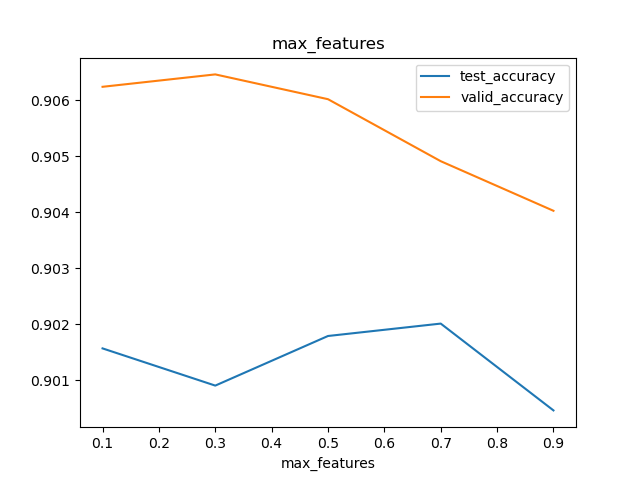
\includegraphics[width=0.6\textwidth]{Q1/output/d_m.png}
  \caption{Plot of the effect of max\_features on the accuracy of the model}
\end{figure}
The accuracy decreases with the increase in max\_features. However, for small increase, the accuracy improves slightly. Therefore, smaller values of max\_features are preferred. The training accuracy increases for larger values of max\_features. Therefore, larger values overfit the model.

\subsubsection{min\_samples\_split}
\begin{figure}[H]
  \centering
  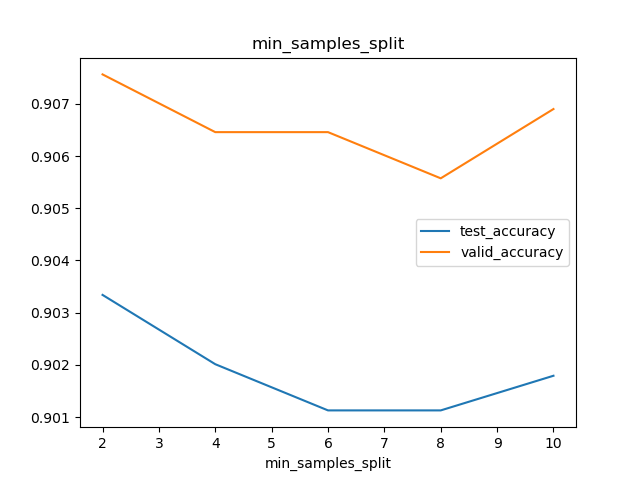
\includegraphics[width=0.6\textwidth]{Q1/output/d_s.png}
  \caption{Plot of the effect of min\_samples\_split on the accuracy of the model}
\end{figure}
The training accuracy decreases with the increase in min\_samples\_split. However, the validation and testing accuracy increases with the increase in min\_samples\_split. Therefore, the model overfits with smaller values of min\_samples\_split.

\newpage

\section{Neural Networks}

\subsection{Sigmoid Activation using a Fixed Learning Rate}
The stopping criteria used is to reach a change in the average cost function across two epochs less than $10^{-8}$ or $1000$ epochs, whicheve happens earlier. When learning, it was observed that for the more complicated neural networks, the epoch criteria was met earlier.\\
The plots and confusion matrices are shown below. It is observed that the model improves when using larger number of perceptrons, however, it slightly drops on using $25$ perceptrons. This is because $1000$ epochs is too less to converge.\\
Additionally, we notice that no model learns the classes $2-9$ at all. This is inferred from the zeroes in all the columns other than the first two in the confusion matrix.

\begin{figure}[H]
  \begin{subfigure}{0.5\textwidth}
    \centering
    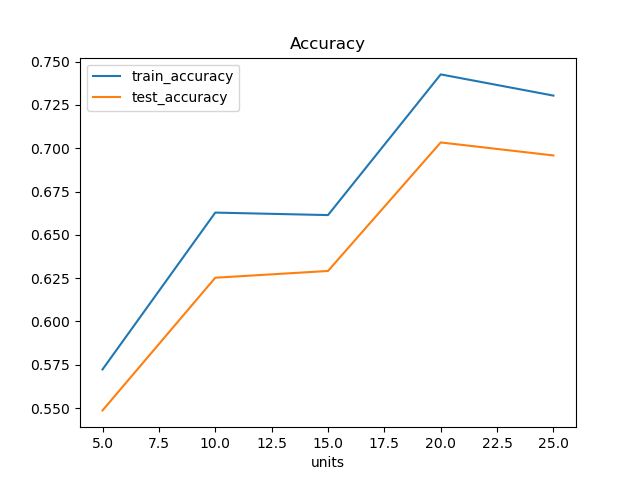
\includegraphics[width=0.9\textwidth]{Q2/output/c_accuracy.png}
    \caption{Plot of the training and test accuracy}
  \end{subfigure}
  \begin{subfigure}{0.5\textwidth}
    \centering
    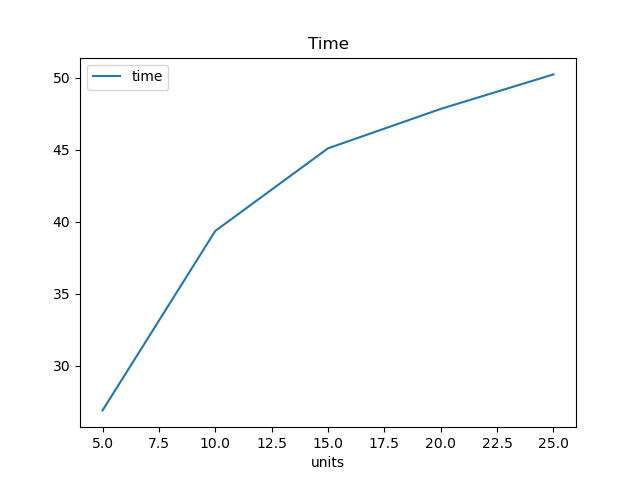
\includegraphics[width=0.9\textwidth]{Q2/output/c_time.png}
    \caption{Plot of the training time}
  \end{subfigure}
\end{figure}

\subsubsection{$5$ Hidden Units}
\begin{equation}
  \begin{split}
    \text{training accuracy} &= 0.5723310675729708\\
    \text{test accuracy} &= 0.548671\\
    \text{confusion matrix} &=
    \begin{pmatrix}
      377431 & 123778 & 0 & 0 & 0 & 0 & 0 & 0 & 0 & 0 \\
      251258 & 171240 & 0 & 0 & 0 & 0 & 0 & 0 & 0 & 0 \\
      21594  & 26028  & 0 & 0 & 0 & 0 & 0 & 0 & 0 & 0 \\
      7397   & 13724  & 0 & 0 & 0 & 0 & 0 & 0 & 0 & 0 \\
      2007   & 1878   & 0 & 0 & 0 & 0 & 0 & 0 & 0 & 0 \\
      1746   & 250    & 0 & 0 & 0 & 0 & 0 & 0 & 0 & 0 \\
      352    & 1072   & 0 & 0 & 0 & 0 & 0 & 0 & 0 & 0 \\
      30     & 200    & 0 & 0 & 0 & 0 & 0 & 0 & 0 & 0 \\
      9      & 3      & 0 & 0 & 0 & 0 & 0 & 0 & 0 & 0 \\
      3      & 0      & 0 & 0 & 0 & 0 & 0 & 0 & 0 & 0
    \end{pmatrix}\\
    \text{training time} &= 39.02067995071411
  \end{split}
\end{equation}

\subsubsection{$10$ Hidden Units}
\begin{equation}
  \begin{split}
    \text{training accuracy} &= 0.6628548580567772\\
    \text{test accuracy} &= 0.625259\\
    \text{confusion matrix} &=
    \begin{pmatrix}
      400963 & 100246 & 0 & 0 & 0 & 0 & 0 & 0 & 0 & 0 \\
      198202 & 224296 & 0 & 0 & 0 & 0 & 0 & 0 & 0 & 0 \\
      11667  & 35955  & 0 & 0 & 0 & 0 & 0 & 0 & 0 & 0 \\
      4343   & 16778  & 0 & 0 & 0 & 0 & 0 & 0 & 0 & 0 \\
      2129   & 1756   & 0 & 0 & 0 & 0 & 0 & 0 & 0 & 0 \\
      1747   & 249    & 0 & 0 & 0 & 0 & 0 & 0 & 0 & 0 \\
      141    & 1283   & 0 & 0 & 0 & 0 & 0 & 0 & 0 & 0 \\
      6      & 224    & 0 & 0 & 0 & 0 & 0 & 0 & 0 & 0 \\
      10     & 2      & 0 & 0 & 0 & 0 & 0 & 0 & 0 & 0 \\
      2      & 1      & 0 & 0 & 0 & 0 & 0 & 0 & 0 & 0
    \end{pmatrix}\\
    \text{training time} &= 53.303688526153564
  \end{split}
\end{equation}

\subsubsection{$15$ Hidden Units}
\begin{equation}
  \begin{split}
    \text{training accuracy} &= 0.6614154338264694\\
    \text{test accuracy} &= 0.629156\\
    \text{confusion matrix} &=
    \begin{pmatrix}
      395803 & 105406 & 0 & 0 & 0 & 0 & 0 & 0 & 0 & 0 \\
      189145 & 233353 & 0 & 0 & 0 & 0 & 0 & 0 & 0 & 0 \\
      11336  & 36286  & 0 & 0 & 0 & 0 & 0 & 0 & 0 & 0 \\
      2809   & 18312  & 0 & 0 & 0 & 0 & 0 & 0 & 0 & 0 \\
      1754   & 2131   & 0 & 0 & 0 & 0 & 0 & 0 & 0 & 0 \\
      1806   & 190    & 0 & 0 & 0 & 0 & 0 & 0 & 0 & 0 \\
      116    & 1308   & 0 & 0 & 0 & 0 & 0 & 0 & 0 & 0 \\
      1      & 229    & 0 & 0 & 0 & 0 & 0 & 0 & 0 & 0 \\
      6      & 6      & 0 & 0 & 0 & 0 & 0 & 0 & 0 & 0 \\
      1      & 2      & 0 & 0 & 0 & 0 & 0 & 0 & 0 & 0
    \end{pmatrix}\\
    \text{training time} &= 59.76480436325073
  \end{split}
\end{equation}

\subsubsection{$20$ Hidden Units}
\begin{equation}
  \begin{split}
    \text{training accuracy} &= 0.7426229508196721\\
    \text{test accuracy} &= 0.703346\\
    \text{confusion matrix} &=
    \begin{pmatrix}
      416637 & 84572  & 0 & 0 & 0 & 0 & 0 & 0 & 0 & 0 \\
      135789 & 286709 & 0 & 0 & 0 & 0 & 0 & 0 & 0 & 0 \\
      3786   & 43836  & 0 & 0 & 0 & 0 & 0 & 0 & 0 & 0 \\
      942    & 20179  & 0 & 0 & 0 & 0 & 0 & 0 & 0 & 0 \\
      2269   & 1616   & 0 & 0 & 0 & 0 & 0 & 0 & 0 & 0 \\
      1787   & 209    & 0 & 0 & 0 & 0 & 0 & 0 & 0 & 0 \\
      1      & 1423   & 0 & 0 & 0 & 0 & 0 & 0 & 0 & 0 \\
      0      & 230    & 0 & 0 & 0 & 0 & 0 & 0 & 0 & 0 \\
      6      & 6      & 0 & 0 & 0 & 0 & 0 & 0 & 0 & 0 \\
      1      & 2      & 0 & 0 & 0 & 0 & 0 & 0 & 0 & 0
    \end{pmatrix}\\
    \text{training time} &= 63.88574767112732
  \end{split}
\end{equation}

\subsubsection{$25$ Hidden Units}
\begin{equation}
  \begin{split}
    \text{training accuracy} &= 0.7303878448620552\\
    \text{test accuracy} &= 0.695839\\
    \text{confusion matrix} &=
    \begin{pmatrix}
      435371 & 65838  & 0 & 0 & 0 & 0 & 0 & 0 & 0 & 0 \\
      162030 & 260468 & 0 & 0 & 0 & 0 & 0 & 0 & 0 & 0 \\
      6315   & 41307  & 0 & 0 & 0 & 0 & 0 & 0 & 0 & 0 \\
      2124   & 18997  & 0 & 0 & 0 & 0 & 0 & 0 & 0 & 0 \\
      2619   & 1266   & 0 & 0 & 0 & 0 & 0 & 0 & 0 & 0 \\
      1857   & 139    & 0 & 0 & 0 & 0 & 0 & 0 & 0 & 0 \\
      20     & 1404   & 0 & 0 & 0 & 0 & 0 & 0 & 0 & 0 \\
      2      & 228    & 0 & 0 & 0 & 0 & 0 & 0 & 0 & 0 \\
      11     & 1      & 0 & 0 & 0 & 0 & 0 & 0 & 0 & 0 \\
      0      & 3      & 0 & 0 & 0 & 0 & 0 & 0 & 0 & 0
    \end{pmatrix}\\
    \text{training time} &= 71.55454468727112
  \end{split}
\end{equation}

\subsection{Sigmoid Activation using an Adaptive Learning Rate}
The stopping criteria used is the same as the previous section. The plots and confusion matrices are given below. It is observed that the accuracy is higher for $5$ units of th hidden layer. However the accuracy is smaller for the other cases. Additionally, the accuracy is lesser for $20$ and $25$ hidden units compares to $10, 15$ hidden units. This is because using the adaptive learning rate slows down the learning and therefore $1000$ epochs is not enough to converge. The training time increases as expected.

\begin{figure}[H]
  \begin{subfigure}{0.5\textwidth}
    \centering
    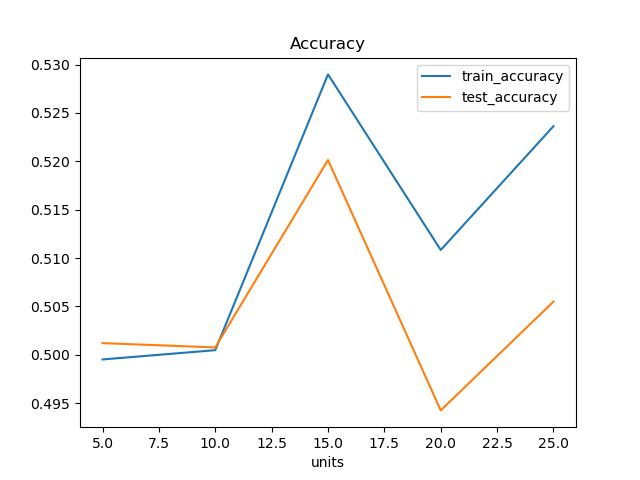
\includegraphics[width=0.9\textwidth]{Q2/output/d_accuracy.png}
    \caption{Plot of the training and test accuracy}
  \end{subfigure}
  \begin{subfigure}{0.5\textwidth}
    \centering
    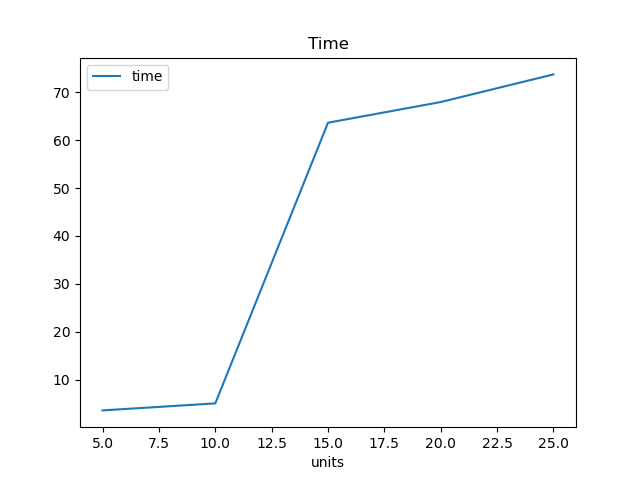
\includegraphics[width=0.9\textwidth]{Q2/output/d_time.png}
    \caption{Plot of the training time}
  \end{subfigure}
\end{figure}

\subsubsection{$5$ Hidden Units}
\begin{equation}
  \begin{split}
    \text{training accuracy} &= 0.589484206317473\\
    \text{test accuracy} &= 0.572393\\
    \text{confusion matrix} &=
    \begin{pmatrix}
      387031 & 114178 & 0 & 0 & 0 & 0 & 0 & 0 & 0 & 0 \\
      237136 & 185362 & 0 & 0 & 0 & 0 & 0 & 0 & 0 & 0 \\
      19466  & 28156  & 0 & 0 & 0 & 0 & 0 & 0 & 0 & 0 \\
      5737   & 15384  & 0 & 0 & 0 & 0 & 0 & 0 & 0 & 0 \\
      1329   & 2556   & 0 & 0 & 0 & 0 & 0 & 0 & 0 & 0 \\
      1678   & 318    & 0 & 0 & 0 & 0 & 0 & 0 & 0 & 0 \\
      251    & 1173   & 0 & 0 & 0 & 0 & 0 & 0 & 0 & 0 \\
      18     & 212    & 0 & 0 & 0 & 0 & 0 & 0 & 0 & 0 \\
      4      & 8      & 0 & 0 & 0 & 0 & 0 & 0 & 0 & 0 \\
      1      & 2      & 0 & 0 & 0 & 0 & 0 & 0 & 0 & 0
    \end{pmatrix}\\
    \text{training time} &= 40.8355929851532
  \end{split}
\end{equation}

\subsubsection{$10$ Hidden Units}
\begin{equation}
  \begin{split}
    \text{training accuracy} &= 0.6117153138744502\\
    \text{test accuracy} &= 0.588626\\
    \text{confusion matrix} &=
    \begin{pmatrix}
      381880 & 119329 & 0 & 0 & 0 & 0 & 0 & 0 & 0 & 0 \\
      215752 & 206746 & 0 & 0 & 0 & 0 & 0 & 0 & 0 & 0 \\
      16304  & 31318  & 0 & 0 & 0 & 0 & 0 & 0 & 0 & 0 \\
      4216   & 16905  & 0 & 0 & 0 & 0 & 0 & 0 & 0 & 0 \\
      2739   & 1146   & 0 & 0 & 0 & 0 & 0 & 0 & 0 & 0 \\
      1761   & 235    & 0 & 0 & 0 & 0 & 0 & 0 & 0 & 0 \\
      210    & 1214   & 0 & 0 & 0 & 0 & 0 & 0 & 0 & 0 \\
      9      & 221    & 0 & 0 & 0 & 0 & 0 & 0 & 0 & 0 \\
      11     & 1      & 0 & 0 & 0 & 0 & 0 & 0 & 0 & 0 \\
      3      & 0      & 0 & 0 & 0 & 0 & 0 & 0 & 0 & 0
    \end{pmatrix}\\
    \text{training time} &= 58.18630528450012
  \end{split}
\end{equation}

\subsubsection{$15$ Hidden Units}
\begin{equation}
  \begin{split}
    \text{training accuracy} &= 0.6239904038384646\\
    \text{test accuracy} &= 0.601769\\
    \text{confusion matrix} &=
    \begin{pmatrix}
      385665 & 115544 & 0 & 0 & 0 & 0 & 0 & 0 & 0 & 0 \\
      206394 & 216104 & 0 & 0 & 0 & 0 & 0 & 0 & 0 & 0 \\
      14607  & 33015  & 0 & 0 & 0 & 0 & 0 & 0 & 0 & 0 \\
      4136   & 16985  & 0 & 0 & 0 & 0 & 0 & 0 & 0 & 0 \\
      2545   & 1340   & 0 & 0 & 0 & 0 & 0 & 0 & 0 & 0 \\
      1792   & 204    & 0 & 0 & 0 & 0 & 0 & 0 & 0 & 0 \\
      180    & 1244   & 0 & 0 & 0 & 0 & 0 & 0 & 0 & 0 \\
      10     & 220    & 0 & 0 & 0 & 0 & 0 & 0 & 0 & 0 \\
      10     & 2      & 0 & 0 & 0 & 0 & 0 & 0 & 0 & 0 \\
      1      & 2      & 0 & 0 & 0 & 0 & 0 & 0 & 0 & 0
    \end{pmatrix}\\
    \text{training time} &= 66.1306664943695
  \end{split}
\end{equation}

\subsubsection{$20$ Hidden Units}
\begin{equation}
  \begin{split}
    \text{training accuracy} &= 0.5859256297481008\\
    \text{test accuracy} &= 0.567364\\
    \text{confusion matrix} &=
    \begin{pmatrix}
      392936 & 108273 & 0 & 0 & 0 & 0 & 0 & 0 & 0 & 0 \\
      248070 & 174428 & 0 & 0 & 0 & 0 & 0 & 0 & 0 & 0 \\
      19182  & 28440  & 0 & 0 & 0 & 0 & 0 & 0 & 0 & 0 \\
      6580   & 14541  & 0 & 0 & 0 & 0 & 0 & 0 & 0 & 0 \\
      2806   & 1079   & 0 & 0 & 0 & 0 & 0 & 0 & 0 & 0 \\
      1809   & 187    & 0 & 0 & 0 & 0 & 0 & 0 & 0 & 0 \\
      273    & 1151   & 0 & 0 & 0 & 0 & 0 & 0 & 0 & 0 \\
      22     & 208    & 0 & 0 & 0 & 0 & 0 & 0 & 0 & 0 \\
      10     & 2      & 0 & 0 & 0 & 0 & 0 & 0 & 0 & 0 \\
      3      & 0      & 0 & 0 & 0 & 0 & 0 & 0 & 0 & 0
    \end{pmatrix}\\
    \text{training time} &= 68.35846948623657
  \end{split}
\end{equation}

\subsubsection{$25$ Hidden Units}
\begin{equation}
  \begin{split}
    \text{training accuracy} &= 0.6100359856057577\\
    \text{test accuracy} &= 0.589734\\
    \text{confusion matrix} &=
    \begin{pmatrix}
      410562 & 90647  & 0 & 0 & 0 & 0 & 0 & 0 & 0 & 0 \\
      243326 & 179172 & 0 & 0 & 0 & 0 & 0 & 0 & 0 & 0 \\
      19587  & 28035  & 0 & 0 & 0 & 0 & 0 & 0 & 0 & 0 \\
      4789   & 16332  & 0 & 0 & 0 & 0 & 0 & 0 & 0 & 0 \\
      3881   & 4      & 0 & 0 & 0 & 0 & 0 & 0 & 0 & 0 \\
      1760   & 236    & 0 & 0 & 0 & 0 & 0 & 0 & 0 & 0 \\
      291    & 1133   & 0 & 0 & 0 & 0 & 0 & 0 & 0 & 0 \\
      9      & 221    & 0 & 0 & 0 & 0 & 0 & 0 & 0 & 0 \\
      12     & 0      & 0 & 0 & 0 & 0 & 0 & 0 & 0 & 0 \\
      3      & 0      & 0 & 0 & 0 & 0 & 0 & 0 & 0 & 0
    \end{pmatrix}\\
    \text{training time} &= 81.43693113327026
  \end{split}
\end{equation}

\subsection{Multiple Hidden Layers: Comparing ReLU and Sigmoid}
The same stopping criteria is used for this part as well.

\subsubsection{ReLU}
\begin{equation}
  \begin{split}
    \text{training accuracy} &= 0.9233106757297082\\
    \text{test accuracy} &= 0.922804\\
    \text{confusion matrix} &=
    \begin{pmatrix}
      500667 & 542    & 0 & 0 & 0 & 0 & 0 & 0 & 0 & 0 \\
      361    & 422137 & 0 & 0 & 0 & 0 & 0 & 0 & 0 & 0 \\
      0      & 47622  & 0 & 0 & 0 & 0 & 0 & 0 & 0 & 0 \\
      0      & 21121  & 0 & 0 & 0 & 0 & 0 & 0 & 0 & 0 \\
      3721   & 164    & 0 & 0 & 0 & 0 & 0 & 0 & 0 & 0 \\
      1984   & 12     & 0 & 0 & 0 & 0 & 0 & 0 & 0 & 0 \\
      0      & 1424   & 0 & 0 & 0 & 0 & 0 & 0 & 0 & 0 \\
      0      & 230    & 0 & 0 & 0 & 0 & 0 & 0 & 0 & 0 \\
      10     & 2      & 0 & 0 & 0 & 0 & 0 & 0 & 0 & 0 \\
      2      & 1      & 0 & 0 & 0 & 0 & 0 & 0 & 0 & 0
    \end{pmatrix}\\
    \text{training time} &= 195.58691668510437
  \end{split}
\end{equation}
Even though the model still doesn't learn classes $2-9$, it does learn the classes $0$ and $1$ highly accurately. In the given training data, about $92\%$ of the training data is in class $0$ and $1$ and the training accuracy is larger than $92\%$, most of which has contribution from these two classes. Therefore, ReLU is a very good choice for the given problem.

\subsubsection{Sigmoid}
\begin{equation}
  \begin{split}
    \text{training accuracy} &= 0.5003998400639744\\
    \text{test accuracy} &= 0.4974\\
    \text{confusion matrix} &=
    \begin{pmatrix}
      482380 & 18829 & 0 & 0 & 0 & 0 & 0 & 0 & 0 & 0 \\
      407478 & 15020 & 0 & 0 & 0 & 0 & 0 & 0 & 0 & 0 \\
      46043  & 1579  & 0 & 0 & 0 & 0 & 0 & 0 & 0 & 0 \\
      20476  & 645   & 0 & 0 & 0 & 0 & 0 & 0 & 0 & 0 \\
      3707   & 178   & 0 & 0 & 0 & 0 & 0 & 0 & 0 & 0 \\
      1879   & 117   & 0 & 0 & 0 & 0 & 0 & 0 & 0 & 0 \\
      1389   & 35    & 0 & 0 & 0 & 0 & 0 & 0 & 0 & 0 \\
      225    & 5     & 0 & 0 & 0 & 0 & 0 & 0 & 0 & 0 \\
      12     & 0     & 0 & 0 & 0 & 0 & 0 & 0 & 0 & 0 \\
      3      & 0     & 0 & 0 & 0 & 0 & 0 & 0 & 0 & 0
    \end{pmatrix}\\
    \text{training time} &= 77.64794874191284
  \end{split}
\end{equation}
The accuracy drops to $50\%$ in this case. The stopping criteria reached in this case was of change in cost function becoming smaller than $10^{-8}$. Thus, we can conclude that the sigmoid derivative is not a very good choice since the backpropagation is smaller.

\subsection{MLPClassifier (Scikit-Learn Library)}
Models were trained for both ReLU and sigmoid activation functions.

\subsubsection{ReLU}
\begin{equation}
  \begin{split}
    \text{training accuracy} &= 0.9999200319872051\\
    \text{test accuracy} &= 0.989527\\
    \text{confusion matrix} &=
    \begin{pmatrix}
      501126 & 5      & 0     & 0     & 75  & 3  & 0   & 0 & 0 & 0 \\
      107    & 422383 & 8     & 0     & 0   & 0  & 0   & 0 & 0 & 0 \\
      565    & 706    & 46328 & 23    & 0   & 0  & 0   & 0 & 0 & 0 \\
      924    & 6      & 163   & 20028 & 0   & 0  & 0   & 0 & 0 & 0 \\
      3694   & 1      & 0     & 0     & 190 & 0  & 0   & 0 & 0 & 0 \\
      1929   & 0      & 0     & 0     & 0   & 67 & 0   & 0 & 0 & 0 \\
      442    & 0      & 94    & 365   & 0   & 0  & 521 & 2 & 0 & 0 \\
      0      & 0      & 0     & 228   & 0   & 0  & 2   & 0 & 0 & 0 \\
      8      & 0      & 0     & 0     & 1   & 3  & 0   & 0 & 0 & 0 \\
      2      & 0      & 0     & 0     & 0   & 1  & 0   & 0 & 0 & 0
    \end{pmatrix}\\
    \text{training time} &= 9.497213125228882
  \end{split}
\end{equation}
The model almost perfectly learns the traning data and performs very well on the test data. The training also happens almost instantly and many folds faster than our training (our model was infact incomplete since the criteria of $1000$ epochs was reached).

\subsubsection{Sigmoid}
\begin{equation}
  \begin{split}
    \text{training accuracy} &= 0.11095561775289885\\
    \text{test accuracy} &= 0.102564\\
    \text{confusion matrix} &=
    \begin{pmatrix}
      378353 & 122856 & 0 & 0 & 0 & 0 & 0 & 0 & 0 & 0 \\
      320188 & 102310 & 0 & 0 & 0 & 0 & 0 & 0 & 0 & 0 \\
      36359  & 11263  & 0 & 0 & 0 & 0 & 0 & 0 & 0 & 0 \\
      16278  & 4843   & 0 & 0 & 0 & 0 & 0 & 0 & 0 & 0 \\
      2865   & 1020   & 0 & 0 & 0 & 0 & 0 & 0 & 0 & 0 \\
      1384   & 612    & 0 & 0 & 0 & 0 & 0 & 0 & 0 & 0 \\
      1096   & 328    & 0 & 0 & 0 & 0 & 0 & 0 & 0 & 0 \\
      172    & 58     & 0 & 0 & 0 & 0 & 0 & 0 & 0 & 0 \\
      9      & 3      & 0 & 0 & 0 & 0 & 0 & 0 & 0 & 0 \\
      2      & 1      & 0 & 0 & 0 & 0 & 0 & 0 & 0 & 0
    \end{pmatrix}\\
    \text{training time} &= 11.053844213485718
  \end{split}
\end{equation}
The accuracy is terrible in this case and much worse than what is learnt by our model. This further proves our claim that ReLU is a much better activation function for the given problem.

\end{document}
